%second chapter of your thesis
\chapter{Hardware}
Onze robot werkt met behulp van 3 zelfgemaakte PCB's. Twee ervan zijn de combinatie van de Motorshield en de Arduino/Atmega328 en de andere is een tussenstuk om de bekabeling te reduceren.





\section{Tussenstuk}
Het tussenstuk is een PCB waarop alle lijnen van de infrarood sensoren toekomen en worden doorgegeven aan de Atmega328. Het voordeel van deze printplaat is dat we nu slechts \'e\'en GND en \'e\'en VCC lijn moeten voorzien tussen de PCB en de Arduino. We hebben op deze PCB ook de mogelijkheid voorzien om de Bluetooth-module en de RFID-reader aan te sluiten. Nadien hebben we ontdekt dat de RFID-reader niet kon worden aangesloten op onze hoofd Arduino waardoor we de RFID-reader ook niet verbonden met dit tussenstuk maar wel rechtstreeks aan de hulp-Arduino. Verbinden met het tussenstuk zou de vereenvoudiging van de bekabeling teniet doen. Het probleem omtrent de RFID-reader leggen we later nog uitgebreider uit. 






We hebben dus tien 5V-aansluitingen voorzien, tien GND-aansluitingen, zes aansluitingen voor de outputsignalen van de sensoren en de pinnen die nodig zijn voor de Bluetooth-module (Key, VCC, GND, TXD, RXD en State). Niet alle zes de uitgangen van de Bluetooth-module moeten worden doorgestuurd naar onze Atmega328. Enkel de signalen VCC, GND, TXD en RXD worden van een uitgang voorzien.  De VCC en de GND aan deze uitgang zorgen voor de voeding van de volledige PCB. We maken gebruik van de HC-05 Bluetooth-module, een foto van de module wordt weergegeven in afbeelding~\ref{fig:HC05}.
\newpage
\begin{figure}[h]
\centering
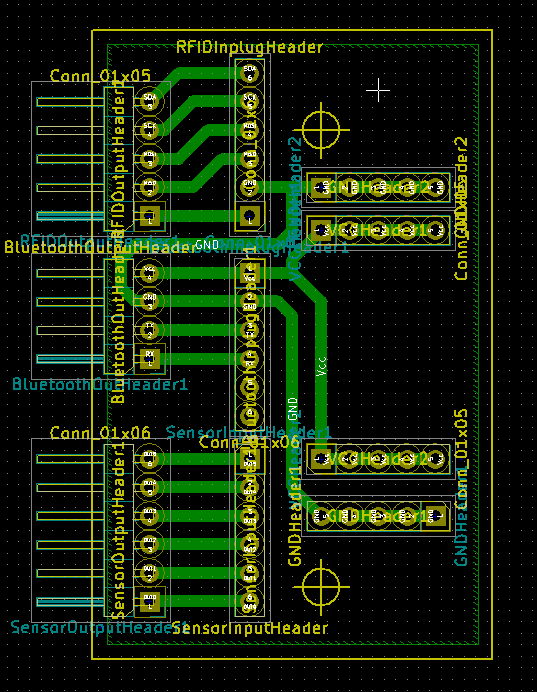
\includegraphics[width=0.3\textwidth]{tussenstukPCB.png}
\caption{Routing van de PCB die als verlengstuk dient. \label{tussenstukPCB}}
\end{figure}


\begin{figure}[h]
\centering
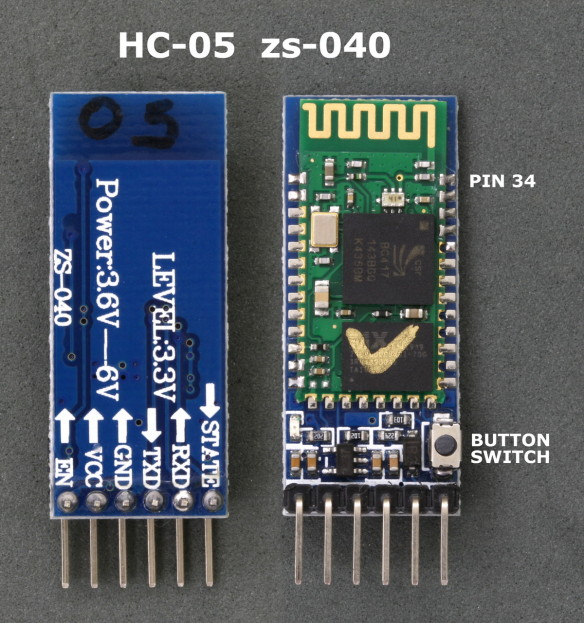
\includegraphics[width=0.3\textwidth]{HC05.jpg}
\caption{De gebruikte Bluetooth-module, ingeplugd op op het tussenstuk}
\label{fig:HC05}
\end{figure}
\section{Arduino met L298}
\subsection{Hulp Arduino}
De tweede printplaat die we ontworpen hebben, is een combinatie van de Atmega328 en de motorshield, hoewel we hier enkel gebruik zullen maken van de Atmega328. De voorzijde van deze PCB kan u zien op Figuur \ref{fig:voorzijde} en de achterzijde op Figuur \ref{fig:achterzijde}. Deze PCB zorgt enkel voor de aansturing en uitlezing van de RFID-reader. We konden de RFID-reader niet aansluiten op onze hoofd Arduino, aangezien de RFID-reader volgende signalen nodig heeft om correct aangestuurd te worden: SS/RX, SCK, MOSI, MISO/TX, IRQ, GND, RST, VCC. 3 van deze pinnen worden ook gebruikt voor de motoraansturing. SCK is namelijk dezelfde pin als die voor de aansturing van de richting van motor B. MOSI is dezelfde pin als die voor de aansturing van de snelheid van motor B. En de laatste overeenkomstige pin is die van MISO, dit is namelijk dezelfde pin als de aansturing van de richting van motor A. Deze pinnen kunnen geen twee signalen gelijktijdig verwerken waardoor we dus opteerden om gebruik te maken van de hulp-Arduino. Een andere mogelijkheid om dit probleem op te lossen kon erin bestaan om gebruik te maken van een RFID-reader die het $I^{2}C$ principe hanteert, in plaats van SPI. Door $I^{2}C$ te gebruiken zouden we geen conflicten met de pinnen gehad hebben waardoor er geen tweede PCB nodig was. We maken gebruik van de MRFC522, dewelke wordt weergegeven in figuur~\ref{fig:MRFC522}. Om een RFID-tag zo goed mogelijk uit te lezen moet de reader op $\approx$ 1 cm boven de tag passeren. We hebben hiervoor zelf een RFID-houder geprint met de 3D-printer zodat deze afstand te allen tijde constant blijft.

\begin{figure}[h]
\centering
\includegraphics[width=0.4\textwidth]{voorzijde.png}
\caption{Voorzijde eigen PCB}
\label{fig:voorzijde}
\end{figure}

\begin{figure}[h]
\centering
\includegraphics[width=0.4\textwidth]{achterzijde.png}
\caption{Achterzijde eigen PCB}
\label{fig:achterzijde}
\end{figure}

\begin{figure}[h]
\centering
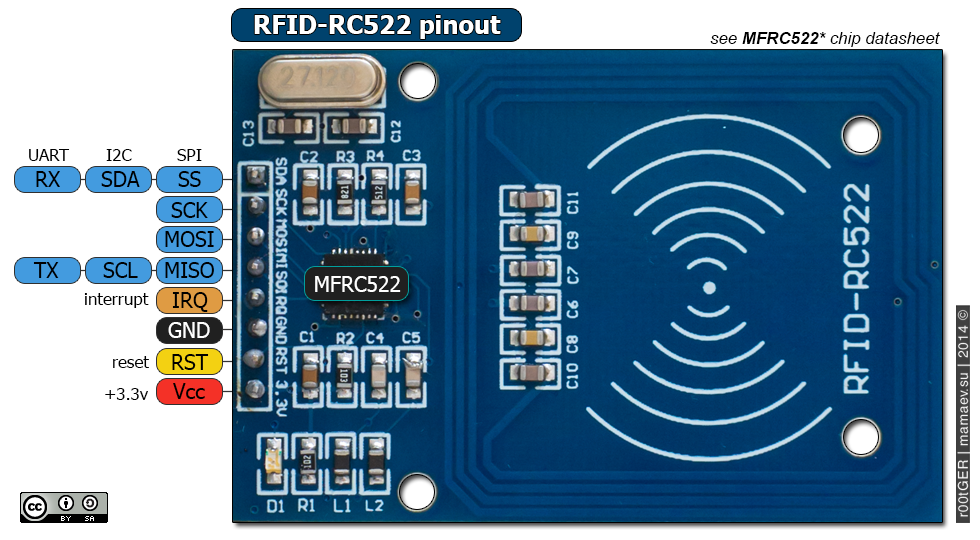
\includegraphics[width=0.4\textwidth]{MRFC522.png}
\caption{Gebruikte RFID-reader MRFC522. \label{fig:MRFC522}}
\label{fig:ACEquiv}
\end{figure}




\subsection{Hoofd Arduino}
Deze PCB is verantwoordelijk voor de aansturing van de motoren en ook voor het doorsturen van de signalen naar de Raspberry Pi via de HC-05 (module verantwoordelijk voor de Bluetooth-communicatie). Deze PCB is identiek aan de hulp Arduino en kan u opnieuw zien op Figuur \ref{fig:voorzijde} en op Figuur \ref{fig:achterzijde}. Het schema kan u raadplegen op Figuur \ref{schema}. Na het finaliseren van de PCB bleken er nog enkele fouten te zijn geslopen in onze versie. Enkele footprints waren aan de kleine kant waardoor sommige componenten slechts heel nipt op de koper-eilandjes pasten. Na ons prototype hadden we deze fout aangepast maar bleek onze correctie nog onvoldoende te zijn om comfortabel te kunnen solderen. Ook een diode bleek bij het testen niet goed gesoldeerd te zijn waardoor we slecht contact kregen wat we opgelost hebben met een externe verbinding. Maar de grootste fout waarop we gestoten zijn, was dat een ingang van de L298 (de IC verantwoordelijk voor de motoraansturing) niet verbonden was met het PWRIN signaal waardoor er geen vermogen naar de motoren gestuurd werd. Dit kwam omdat er een hi\"erarchical label ontbrak in ons schema op de betreffende locatie aan de L298. We hebben dit probleem kunnen oplossen door een extra kabel te solderen van het PWRIN signaal naar de betreffende pin van de L298. \\
Als vertrekpunt hadden we het schema van een een Arduino Uno ter beschikking op het internet. Als eerste konden we de USB-interface voor de aansluiting van een USB-kabel weglaten aangezien we dit in ons finaal ontwerp niet nodig hadden. Deze USB-interface wordt weergegeven in figuur~\ref{fig:USB-interface}.
\begin{figure}[h]
\centering
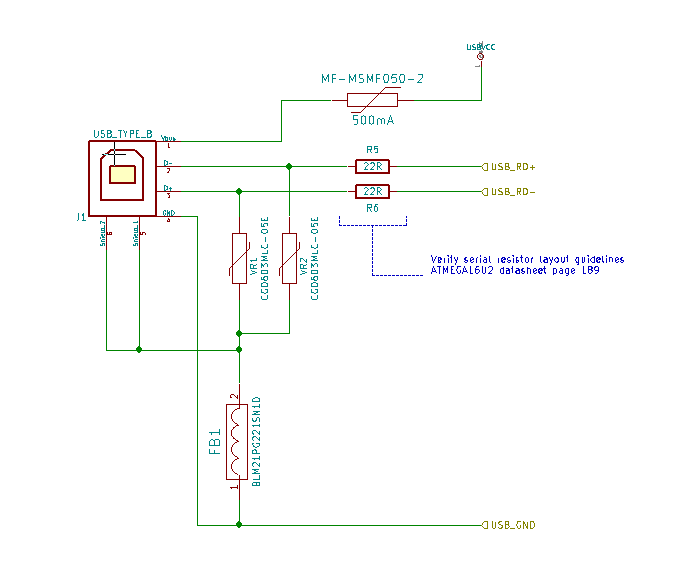
\includegraphics[width=0.5\textwidth]{USB_Interface.png}
\caption{USB interface die we weg hebben gelaten}
\label{fig:USB-interface}
\end{figure}
Voor het uploaden van een programma maken we dan gebruik van de ICSP-pinnen die we nauwkeurig verbinden met een andere Arduino die de code doorstuurt.  Alle LED's die normaal gezien aanwezig zijn op de Arduino Uno hebben we  weggelaten omdat we dit niet echt nodig hebben en dit onze Arduino groter zou maken dan nodig. Een voorbeeld van een LED die we weggelaten hebben wordt weergegeven in figuur~\ref{fig:regulator}. Om het ons eenvoudiger te maken, pasten we in het schema ook de namen van de labels aan naar meer betekenisvollere namen zodat we de namen van de lijnen zo eenvoudiger konden interpreteren. Zo veranderden we bijvoorbeeld MISO door DIR A aangezien deze lijn verantwoordelijk was voor de richting van Motor A. R8 hebben we ook weggelaten aangezien dit een weerstandswaarde van 0 $\Omega$ heeft. Deze weerstand wordt voornamelijk gebruikt als brug om er banen onder te kunnen trekken. Pinnen 27 en 28 hebben we niet nodig, dus mogen we de condensator verwijderen. De jumper hebben we weggelaten omdat we die niet nodig achtten. Dit alles wordt weergegeven in figuur~\ref{fig:atmega}. Eenmaal het schema klaar was, konden we starten met het routen van de printbanen. De afmetingen van de PCB bedragen (52,324mm x 61.468mm). De uiteindelijke grootte van de printplaat bedraagt 53.34mm x 73.152mm, zodat de bevestigingsgaten van de PCB overeenkomen met de vijzen van het chassis.  De breedte van de printbanen van onze oorspronkelijke routing bedroeg 10 mills(= 0.254mm). Aangezien dit zeer smal was en de kans groot was dat er een baan wegge\"etst zou worden, hebben we zoveel mogelijk banen verbreed tot 30 mills. De breedte van de printbanen en de diameters van de drills, worden weergegeven in tabel~\ref{table:afmetingen}.\\
\begin{figure}[h]
\centering
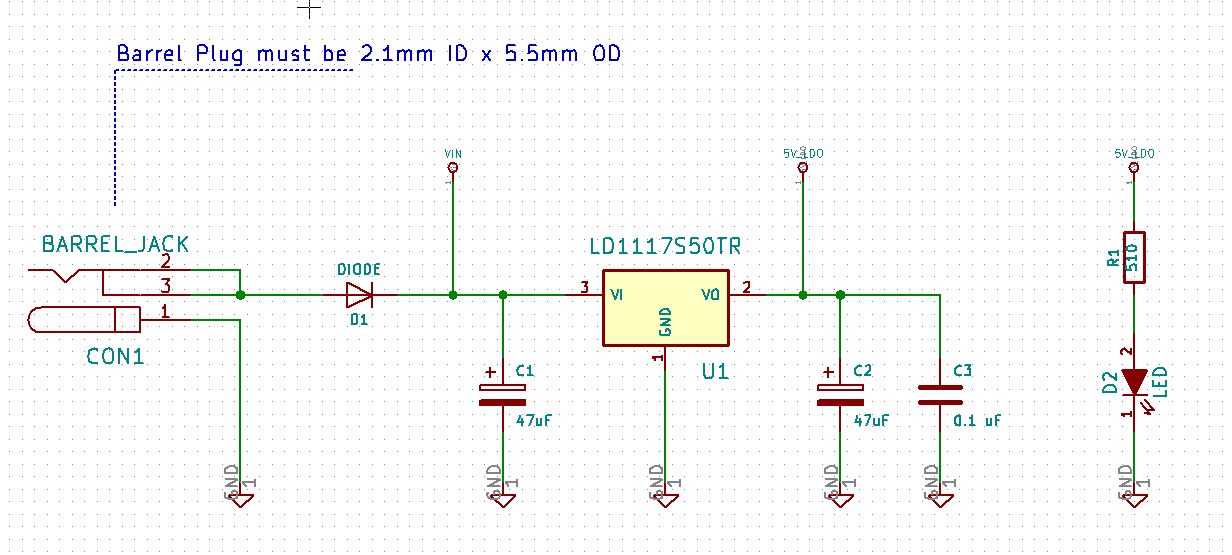
\includegraphics[width=0.5\textwidth]{Voltage_Regulator.png}
\caption{Voorbeeld van LED die we weggelaten hebben}
\label{fig:regulator}
\end{figure}

\begin{figure}[h]
\centering
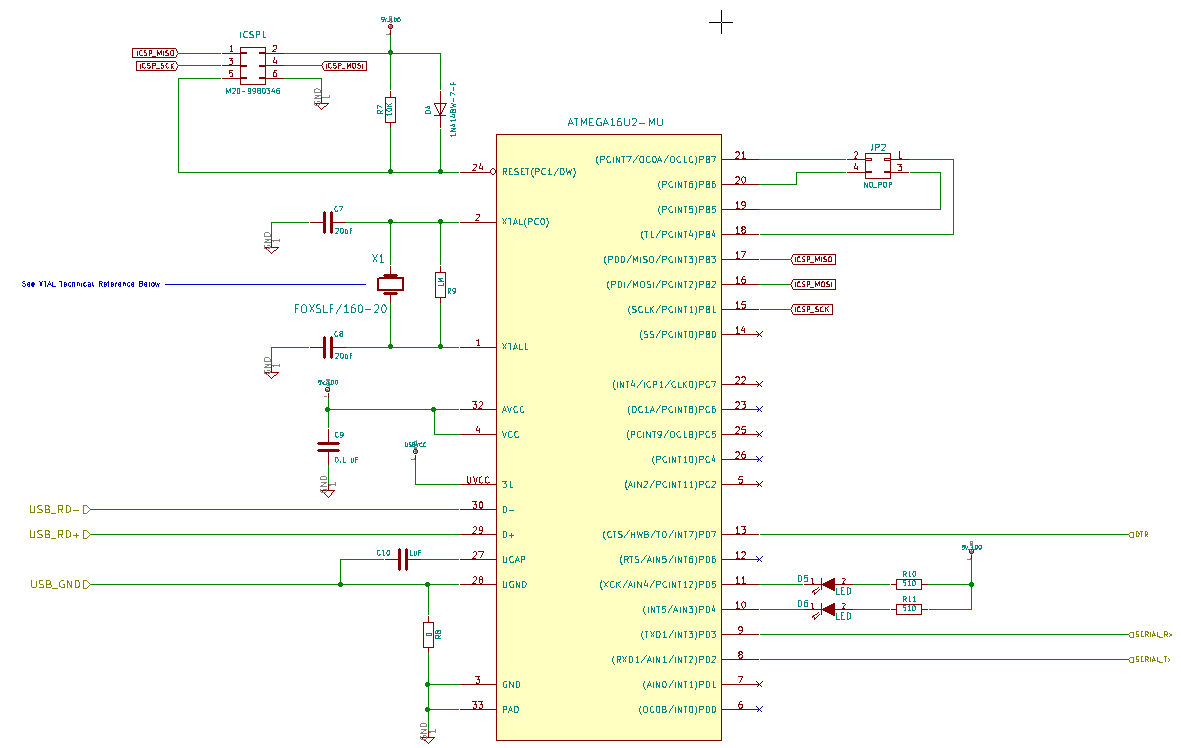
\includegraphics[width=0.5\textwidth]{Atmega.png}
\caption{Voorbeeld van weerstand die we weggelaten hebben rond de Atmega328}
\label{fig:atmega}
\end{figure}

\begin {table}[H]
\caption {Tabel afmetingen koperbanen.} \label{table:afmetingen}
	\begin{center}
	\begin{tabular}{ | l | l | l | l | l |}
	\hline
	  & Clearance & Track Width & Via Dia & Via Drill\\ \hline
	Default & 0.25 & 0.25 & 0.6 & 0.4\\ \hline
	0.5 & 0.25 & 0.5 & 0.7 & 0.5 \\ \hline
	12 mills & 0.25 & 0.3 & 0.6 & 0.4 \\ \hline
	15 mills & 0.25 & 0.38 & 0.6 & 0.4 \\ \hline
	30 mills & 0.25 & 1 & 0.6 & 0.4 \\ \hline
	\end{tabular}
	\end{center}
\end{table}
 Enkele banen hebben een breedte van maximaal 15 mills, aangezien de printplaat zodanig compact gemaakt was dat nog meer verbreden geen optie was. \'E\'en van onze uitdagingen was om de printplaat te voorzien van zo weinig mogelijk via's, wat we konden minimaliseren tot 20, op de hele PCB. Bij de  eerste pogingen om de printplaat te etsen, stootten we op het probleem dat de fijnste banen oplosten waardoor er niet langer verbinding was. We kregen de tip om gebruik te maken van een kopervlak, zodat de PCB minder lang in het zuurbad moest liggen bij het etsen. Achteraf gezien konden we beide vlakken gebruiken als bijvoorbeeld een GND-vlak, wat in ons ontwerp niet is toegepast. De routing van voor- en achterkant wordt weergegeven in figuren~\ref{fig:front} en~\ref{fig:back}. Er moet wel bij verteld worden dat we per ongeluk de zijden omgewisseld hebben, de Back-zijde op KiCad is voor ons de voorkant en vice versa. Achteraf gezien gaf dit toch enkele problemen omdat we altijd in spiegelbeeld moesten redeneren. Dit zullen we in het vervolg dus proberen te vermijden. Eens de PCB volledig bestukt was, wilden we deze eerst testen met een standaardprogramma voor de Atmega nl. Blink-Led. Dit programma werkte onmiddellijk waardoor we verkeerdelijk veronderstelden dat de hele PCB correct was. We bespreken dit uitgebreid in het hoofdstuk~\ref{Moeilijkheden}. De volledige praktische PCB wordt weergegeven in figuren~\ref{fig:achterkantPCB} en~\ref{fig:voorkantPCB}. 
\begin{figure}[h]
\centering
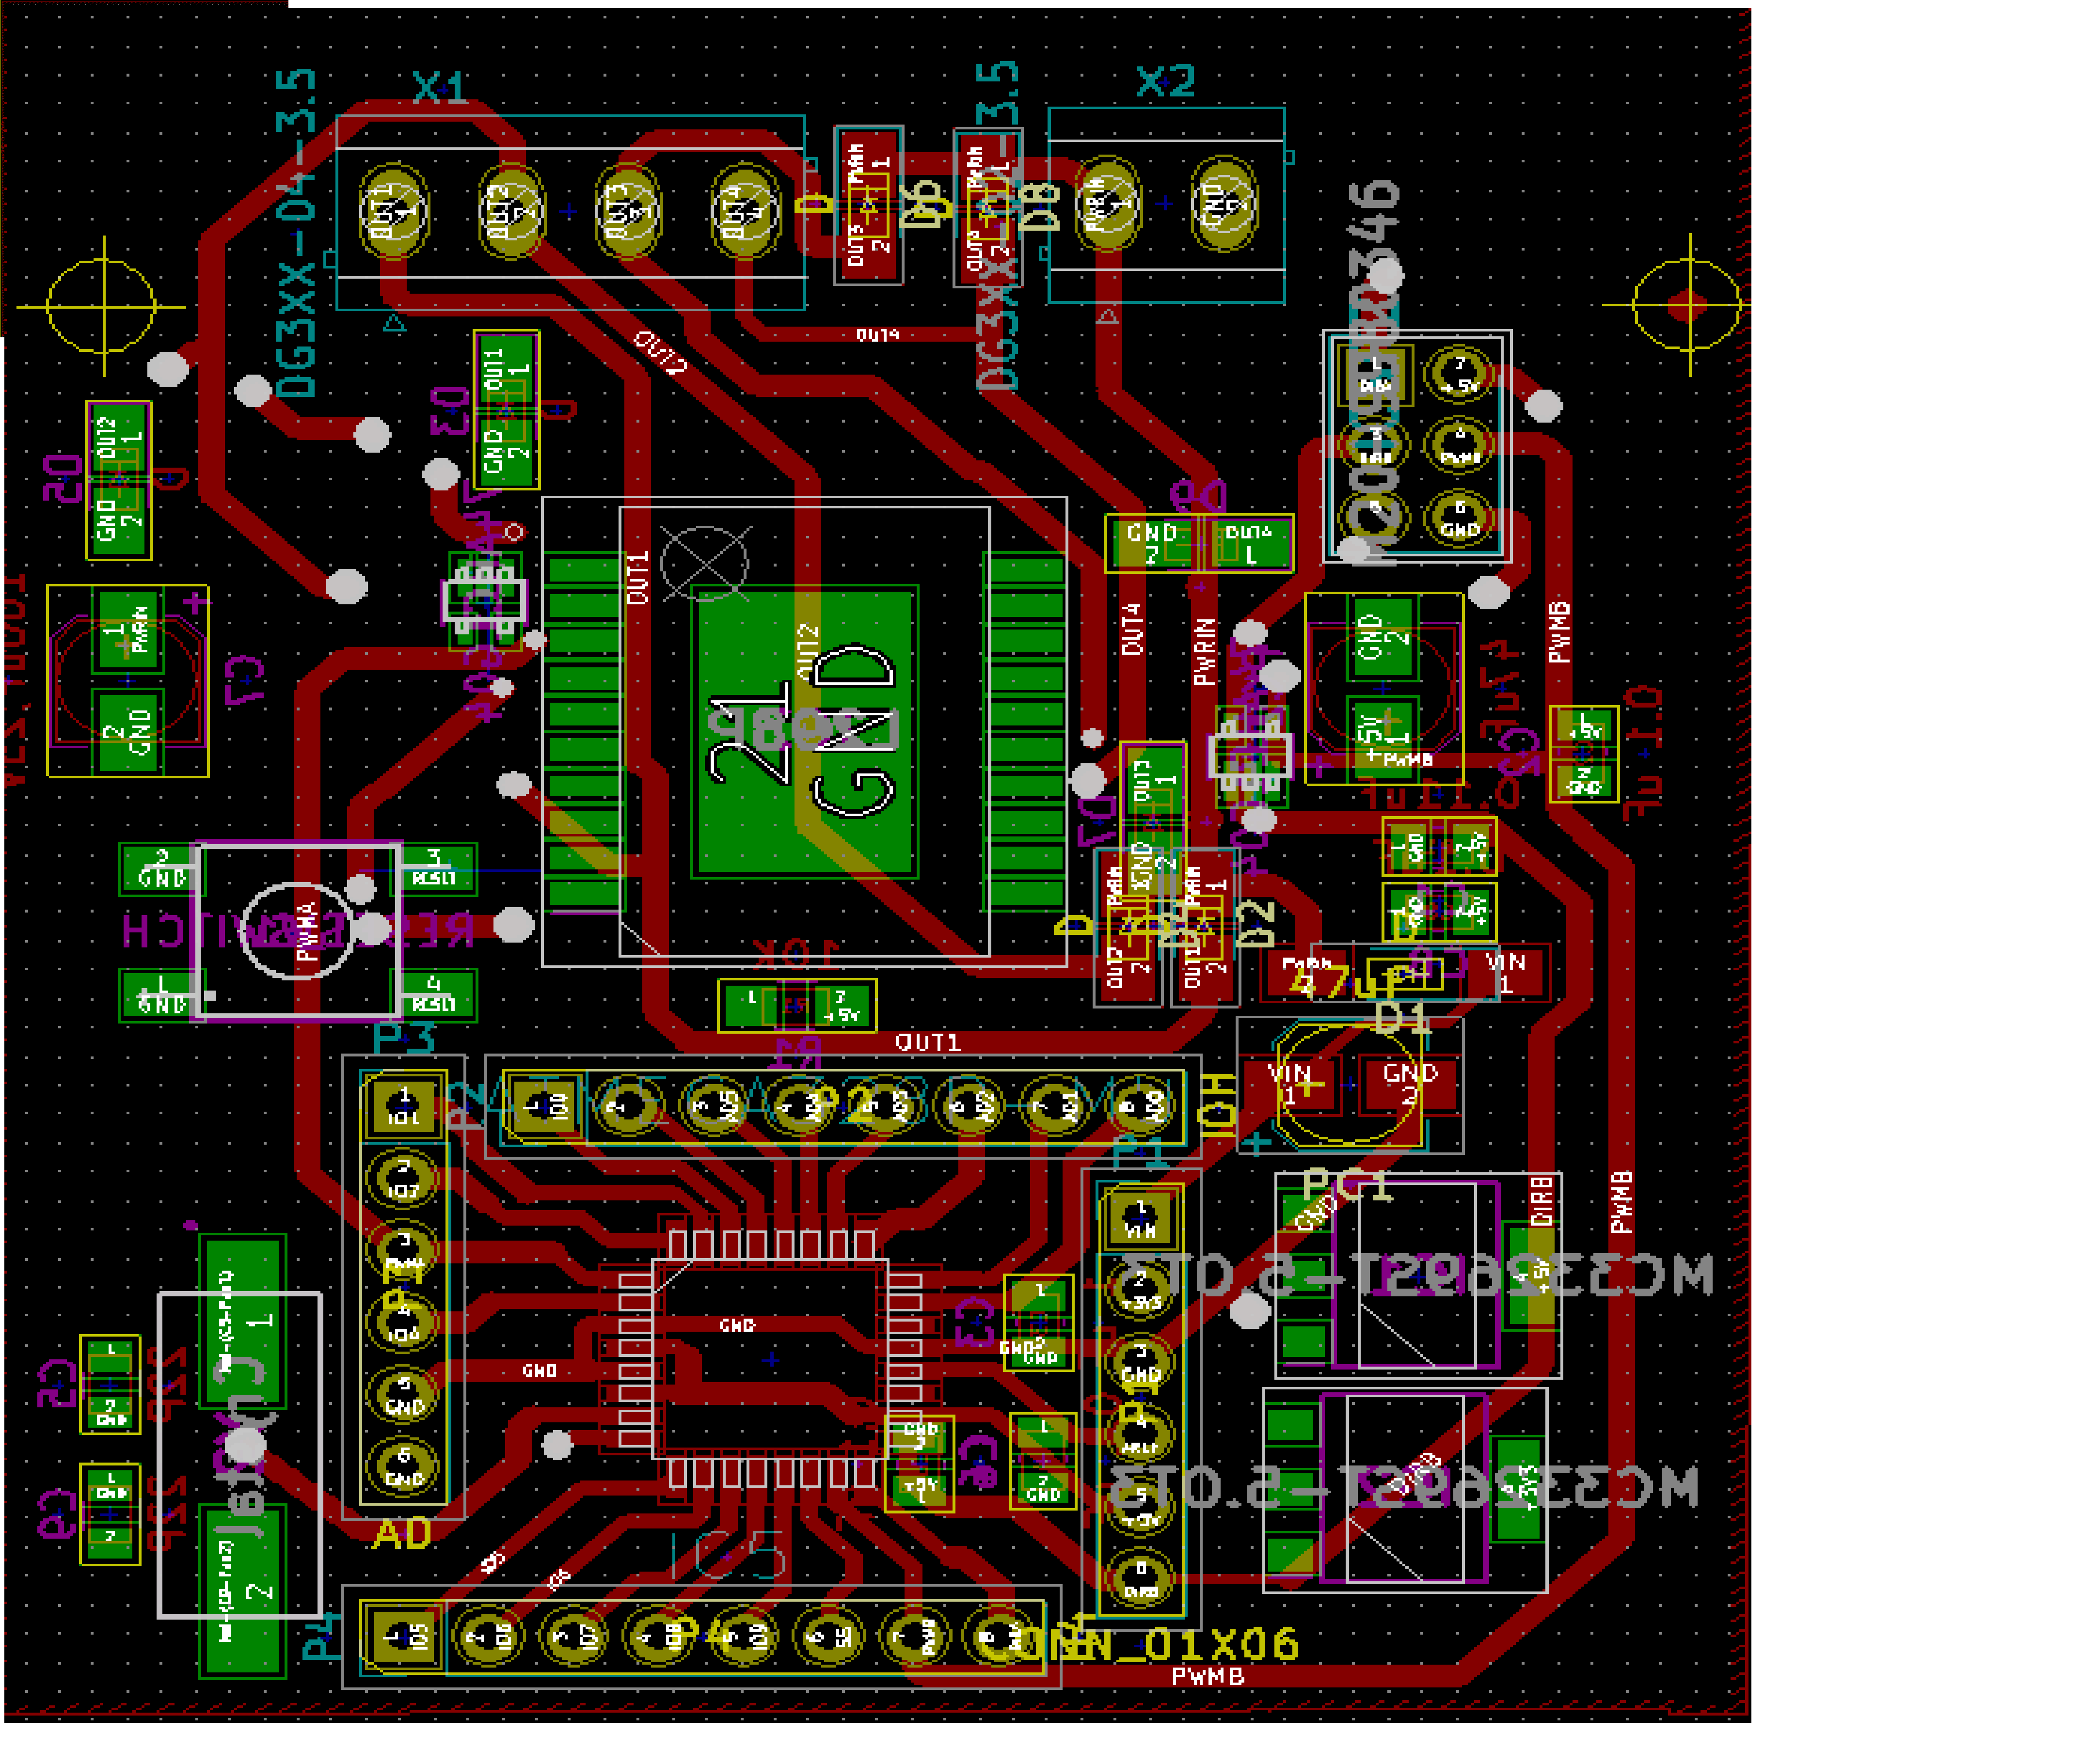
\includegraphics[width=0.5\textwidth]{Front.png}
\caption{Front banen van onze eigen PCB (= onderkant voor ons)}
\label{fig:front}
\end{figure}

\begin{figure}[h]
\centering
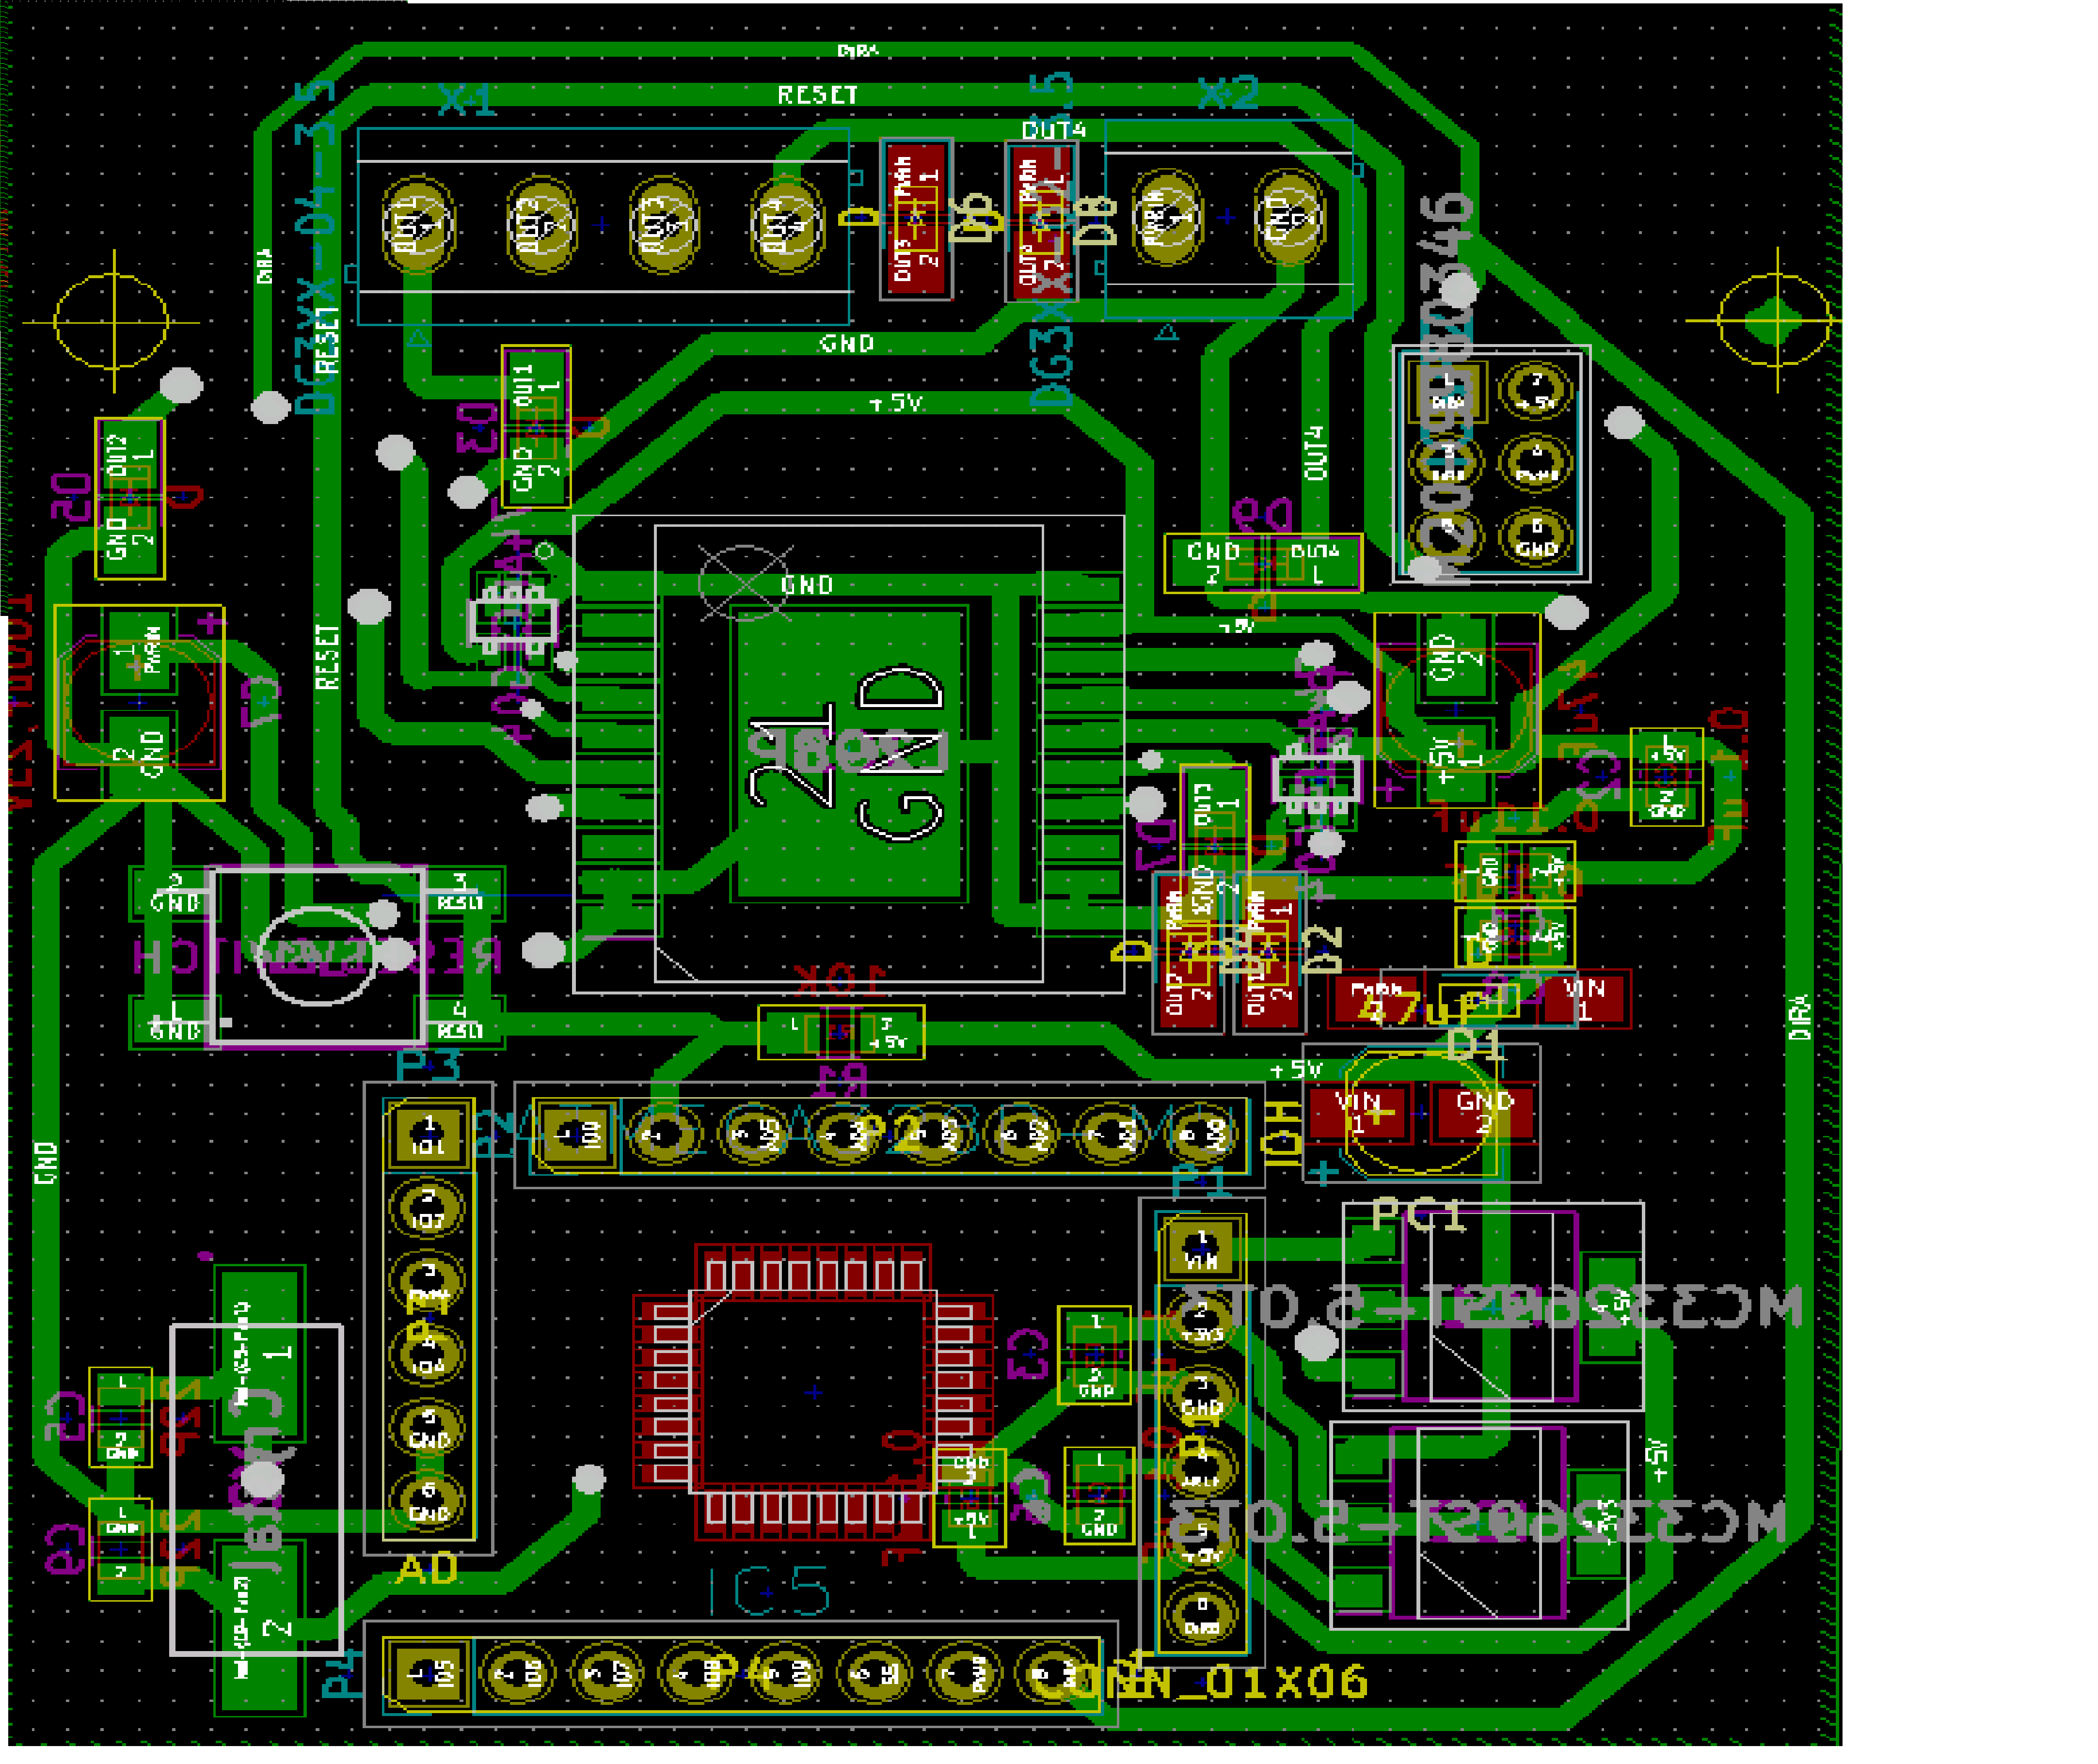
\includegraphics[width=0.5\textwidth]{Back.png}
\caption{Back banen van onze eigen PCB (= bovenkant voor ons)}
\label{fig:back}
\end{figure}

\begin{figure}[h]
\centering
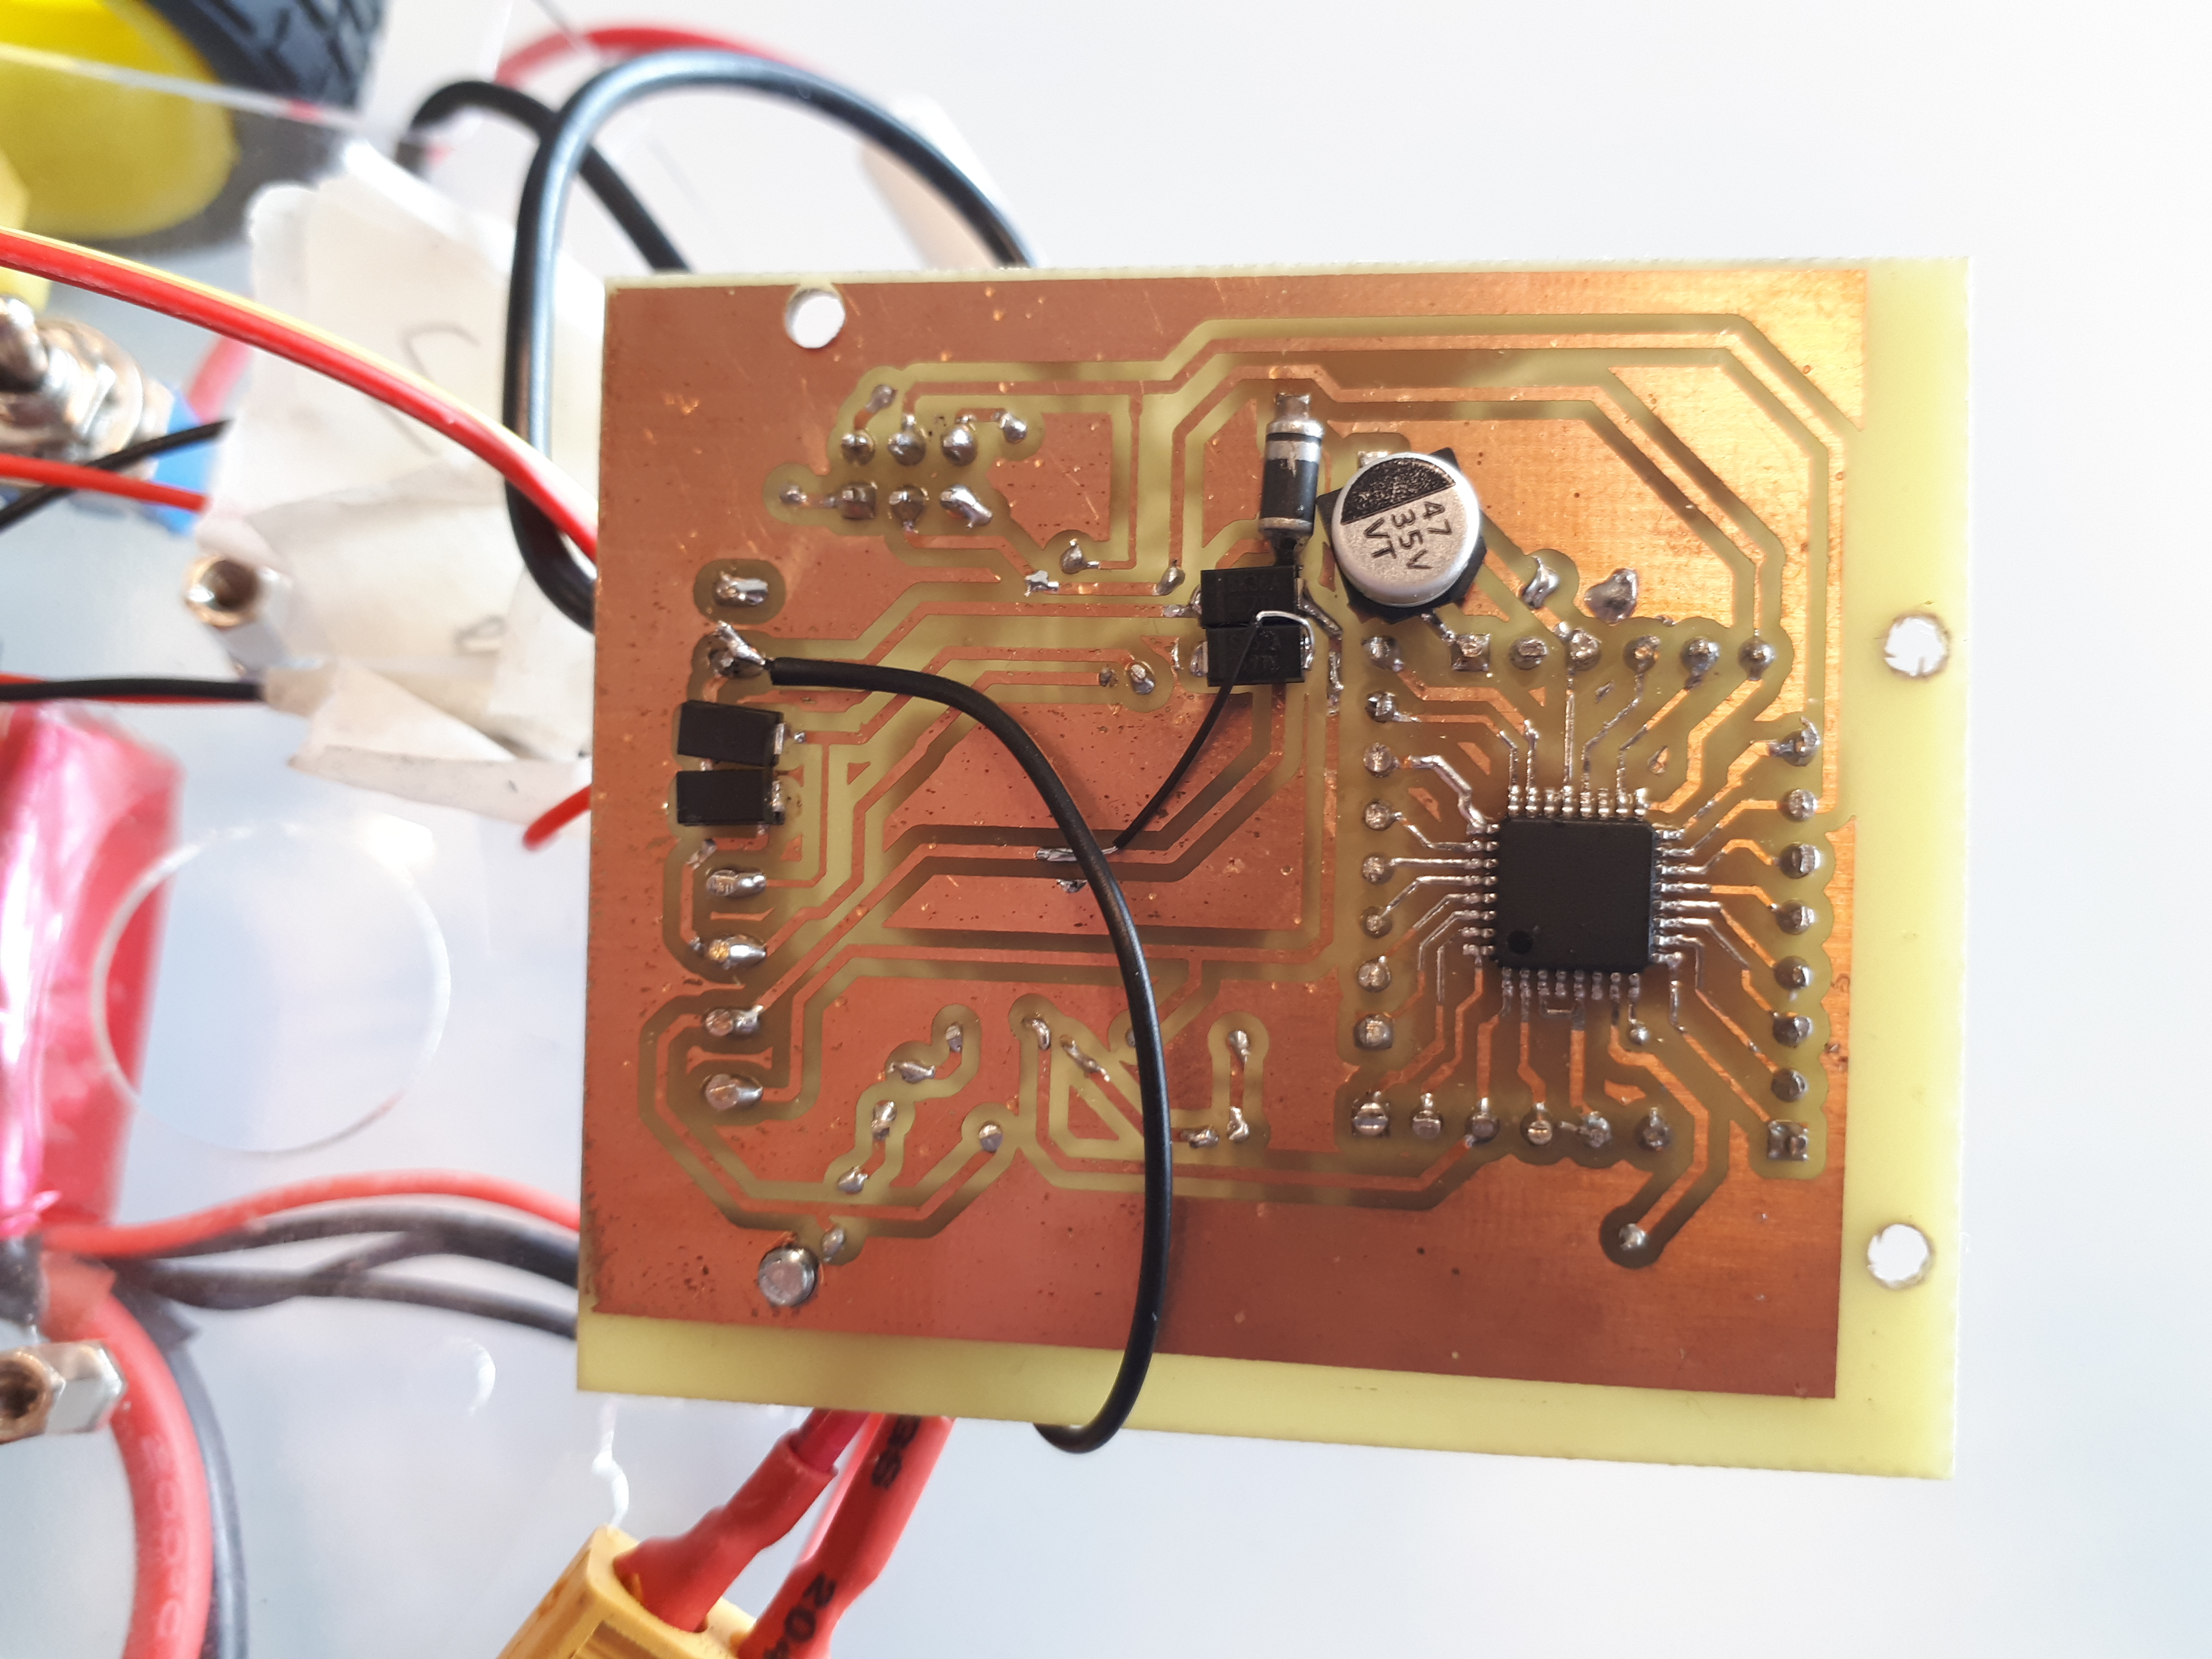
\includegraphics[width=0.6\textwidth]{AchterkantPCB.jpg}
\caption{Eindresultaat achterkant PCB}
\label{fig:achterkantPCB}
\end{figure}

\begin{figure}[h]
\centering
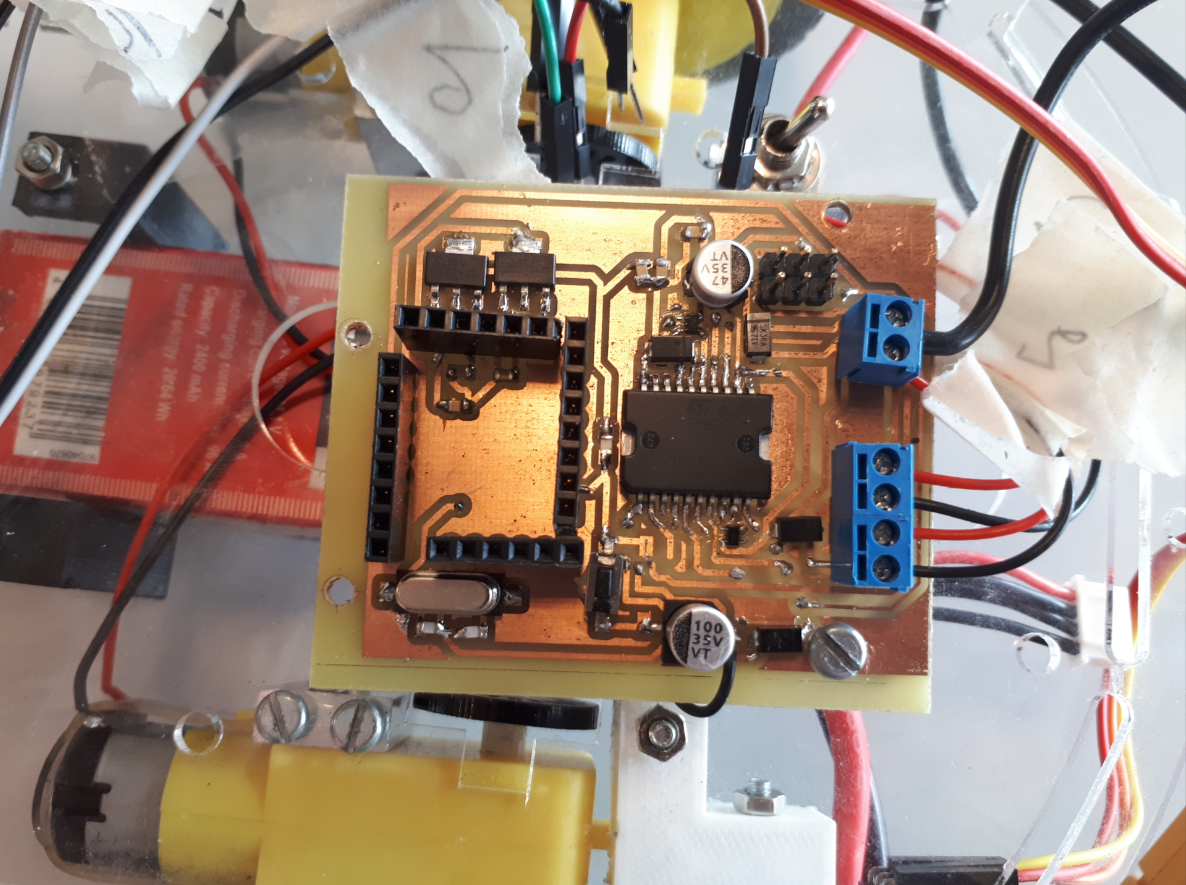
\includegraphics[width=0.6\textwidth]{VoorkantPCB.jpg}
\caption{Eindresultaat voorkant PCB}
\label{fig:voorkantPCB}
\end{figure}

\begin{figure}[h]
\centering
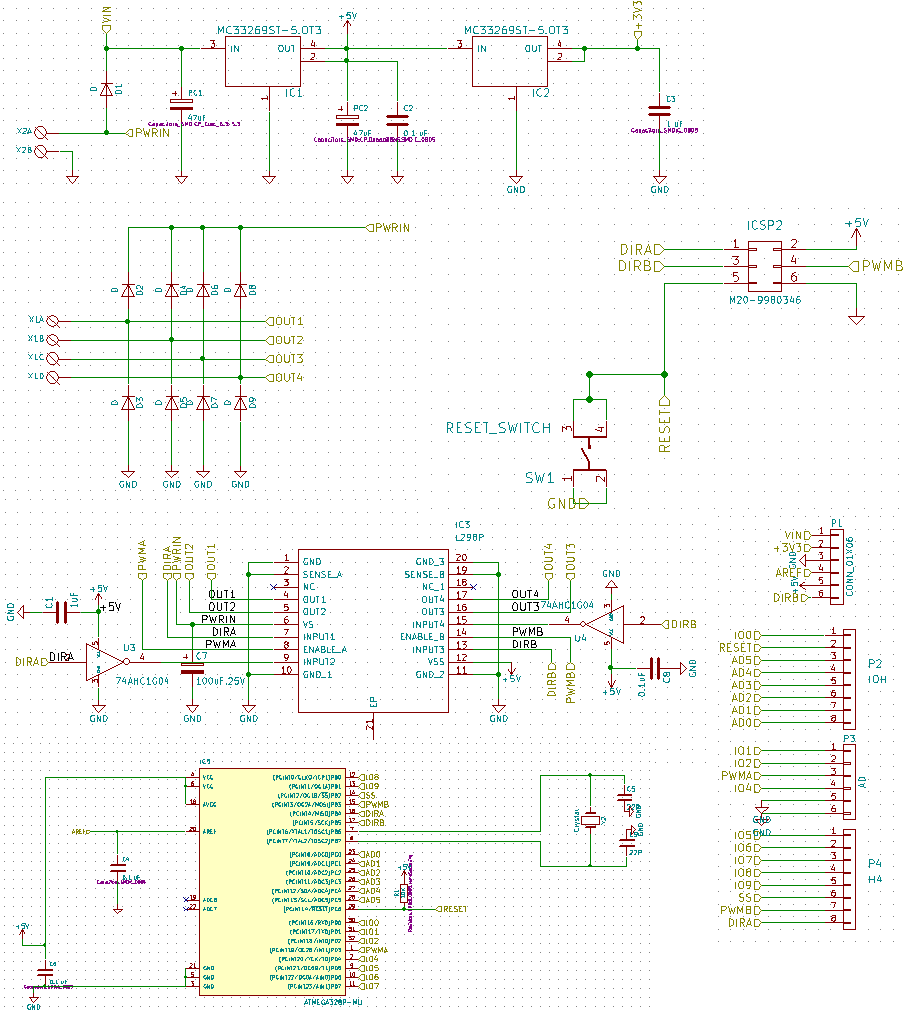
\includegraphics[width=1\textwidth]{volledigschema}
\caption{Volledig schema van de hoofd- en hulp-Arduino}
\label{schema}
\end{figure}
%In het vorig hoofdstuk hebben we naar deze tekst verwezen\label{verwijzing}.
